\section{Auswertung}

In der folgenden Auswertung werden die verschiedenen aufgenommenen Spektren
ausgewertet, um die Eigenschaften des Detektors zu bestimmen, sowie zwei verschiedene
unbekannte Quellen zu klassifizieren. Dafür werden verschiedene \textsc{Python}-Pakete
verwendet. Es handelt sich um die Pakete \textsc{uncertainties} für die Fehlerrechnung,
\textsc{scipy.optimize} für die Bestimmung der verschiedenen Peaks sowie
\textsc{curve\_{fit}} für die Ausgleichsrechnungen.

\subsection{Kalibrierung des Detektors mit einer $^{152}\ce{Eu}$-Quelle}

Zu Beginn des Experimentes wird eine Kalibrierung des Detektors mithilfe
einer $^{152}\ce{Eu}$-Probe durchgeführt. Anhand des Spektrums werden dann mithilfe
bekannter Energien des Gamma-Spektrums die Transformation der Kanäle in die
entsprechenden Energien sowie die Parameter für die Effizienz in Abhängigkeit
der Energie bestimmt. Die Messung wurde in einem Zeitraum von
$t\ua{ges} = \SI{3393}{\second}$ durchgeführt.

\subsubsection{Bestimmung der Energie-Transformation}
\label{subsubsec:Eu}

\begin{figure}
  \centering
  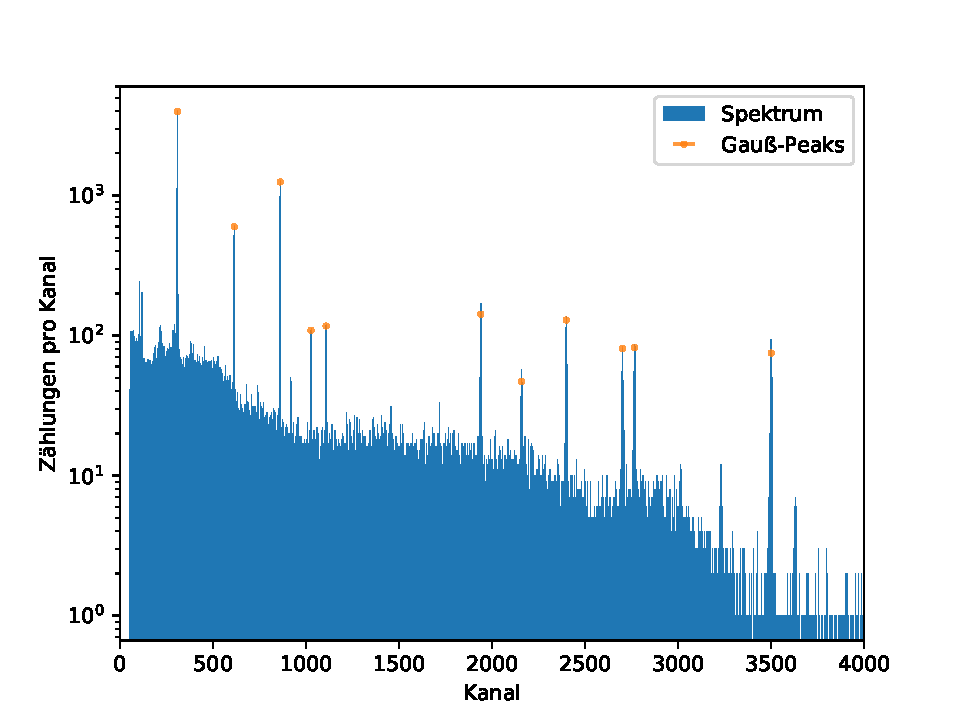
\includegraphics[width = 0.85\textwidth]{Python/Plots/Europium.pdf}
  \caption{Aufgenommenes Spektrum der $^{152}\ce{Eu}$-Quelle. Die bestimmten
  Vollenergiepeaks sind farblich markiert.}
  \label{fig:EuSpek}
\end{figure}
In Abbildung~\ref{fig:EuSpek} ist das aufgenommene Spektrum für
$^{152}\ce{Eu}$ dargstellt. Um den einzelnen Kanälen eine Energie zuordnen
zu können, werden die Kanäle der verschiedenen Peaks mit \textsc{scipy.optimize.find\_{peaks}}
bestimmt. Anschließend wird jeweils in einem Bereich von $\pm \num{30}$ Kanälen
um die bestimmten Kanäle eine
Anpassung mit der folgenden Gauß-Funktion durchgeführt:
\begin{equation}
  N(x) = A\cdot exp{\left( \frac{x-\mu}{\sigma}\right)^2} + B.
  \label{eqn:Gausfit}
\end{equation}
Die einzelnen Parameter sind in Tabelle~\ref{tab:EuGauß} eingetragen und die bestimmte
Mittelwerte der Peaks sind in Abbildung~\ref{fig:EuSpek} dargestellt. Jedem
Peak wird dabei eine der charakteristischen Energien aus dem Gamma-Spektrum
von $^{152}\ce{Eu}$ zugeordnet. Mithilfe der gefitteten Mittelwerte $\mu$ kann
nun die Transformation der Kanäle in die zugehörigen Energiewerte bestimmt werden.
Dafür werden die Energien $E_{\gamma, \text{lit}}$ an die bestimmten Kanäle $\mu$ gemäß
einer linearen Funktion der Form
\begin{equation}
  E(x) = m \cdot x + b
\end{equation}
angepasst. Dabei ergeben sich die folgenden Parameter:
\begin{align}
  m &= \SI{0.40299(6)}{\kilo\eV\per\text{Kanalnummer}} \\
  b &= \SI{-2.76(11)}{\kilo\eV}.
\end{align}
\begin{table}
  \centering
  \caption{Bestimmte Anpassung-Parameter der Gaußfunktion für das $^{152}\ce{Eu}$-Spektrum.}
  \label{tab:EuGauß}
  \begin{tabular}{S[table-format=4] S[table-format=4]@{${}\pm{}$} S[table-format=2]
    S[table-format=4.2]@{${}\pm{}$} S[table-format=1.2]
    S[table-format=1.2]@{${}\pm{}$} S[table-format=1.2]
    S[table-format=2.0]@{${}\pm{}$} S[table-format=1] }
    \toprule
    {Kanal} & \multicolumn{2}{c}{$A$ / Zählung} & \multicolumn{2}{c}{$\sigma$ / Kanal}
    & \multicolumn{2}{c}{$\mu$ / Kanal} & \multicolumn{2}{c}{$B$ / Zählung}\\
    \midrule
     309 & 3926 & 18 &  309.84 & 0.01 & 1.14 & 0.01 & 77 & 2 \\
     614 &  583 &  7 &  613.92 & 0.02 & 1.36 & 0.02 & 33 & 1 \\
     861 & 1223 &  7 &  860.97 & 0.01 & 1.54 & 0.01 & 18 & 1 \\
    1027 &   86 &  3 & 1026.94 & 0.06 & 1.43 & 0.06 & 14 & 1 \\
    1108 &  100 &  3 & 1108.18 & 0.05 & 1.53 & 0.05 & 15 & 1 \\
    1939 &  157 &  4 & 1939.58 & 0.07 & 2.51 & 0.07 & 10 & 1 \\
    2160 &   42 &  2 & 2159.17 & 0.16 & 2.78 & 0.16 & 10 & 1 \\
    2393 &  124 &  3 & 2398.89 & 0.08 & 3.08 & 0.08 &  6 & 1 \\
    2702 &   67 &  3 & 2701.66 & 0.14 & 3.22 & 0.15 &  6 & 1 \\
    2765 &   84 &  2 & 2766.44 & 0.09 & 3.36 & 0.09 &  5 & 1 \\
    3500 &   89 &  2 & 3501.07 & 0.11 & 3.99 & 0.12 &  1 & 1 \\
    \bottomrule
  \end{tabular}
\end{table}


Die verwendeten Kanalnummern, die dazugehörigen Literaturwerte der Energien
$E_{\gamma, \text{lit}}$ sowie die mit der Transformation bestimmten Energien
$E_{\gamma, \text{exp}}$ sind in Tabelle~\ref{tab:Kalibrierung} eingetragen. In Abbildung
\ref{fig:Kalibrierung} sind die Datenpunkte sowie der dazugehörige Fit
grafisch dargestellt. Die bestimmten Parameter werden in den folgenden Abschnitten
verwendet, um das Spektrum direkt in Abhängigkeit von der Energie darzustellen.
\begin{figure}
  \centering
  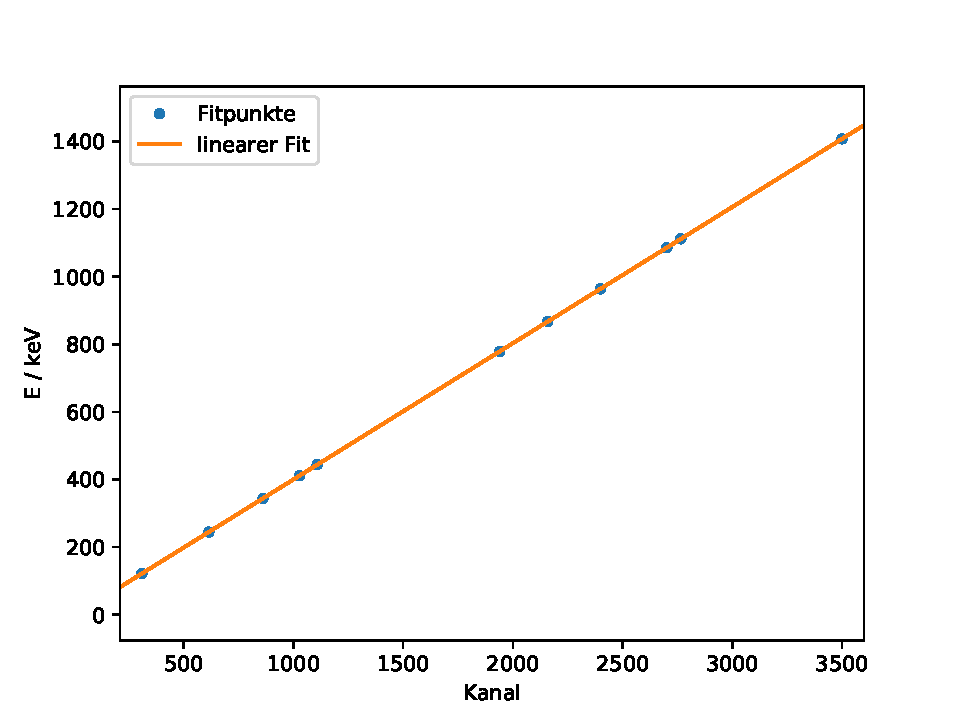
\includegraphics[width = 0.85\textwidth]{Python/Plots/Kalibrierung.pdf}
  \caption{Verwendte Datenpunkte für die Energiekalibrierung sowie der bestimmte
  lineare Fit für $^{152}\ce{Eu}$.}
  \label{fig:Kalibrierung}
\end{figure}
\begin{table}
  \centering
  \caption{Die Kanäle mit den dazugehörigen Literaturwerten und den Energien aus der linearen Regression.}
  \label{tab:Kalibrierung}
  \begin{tabular}{S[table-format=4] S[table-format=4.2] S[table-format=4.2]@{${}\pm{}$} S[table-format=1.2]}
    \toprule
    {$\mu$ / Kanal} & {$E_{\gamma, \text{lit}} $ / $\si{\kilo\eV}$ } & \multicolumn{2}{c}{$E_{\gamma, \text{exp}} $ / $\si{\kilo\eV}$ } \\
    \midrule
     309 &  121.78 &  121.76  & 0.11  \\
     614 &  244.40 &  244.67  & 0.12  \\
     861 &  344.40 &  344.21  & 0.12  \\
    1027 &  411.12 &  411.11  & 0.13  \\
    1108 &  443.96 &  443.75  & 0.13  \\
    1940 &  778.90 &  778.63  & 0.16  \\
    2159 &  867.37 &  867.70  & 0.16  \\
    2399 &  964.08 &  961.60  & 0.17  \\
    2702 & 1085.90 & 1086.12  & 0.19  \\
    2766 & 1112.20 & 1111.51  & 0.19  \\
    3501 & 1408.00 & 1407.71  & 0.23  \\
    \bottomrule
  \end{tabular}
\end{table}


\subsubsection{Bestimmung der Parameter für die Effizienz}
\label{subsubsec:Eff}

Die Nachweiswahrscheinlichkeit der Gamma-Quanten ist im Allgemeinen von der Energie
abhängig, weshalb im Folgenden eine Funktion für die Effizienz in Abhängigkeit von
der Energie bestimmt werden soll. Dafür muss zuerst die Aktivität der Probe
bestimmt werden. Es ist bekannt, dass die Aktivität der Probe am 01.10.2000
$A\ua{0} = \SI{4130(60)}{\becquerel}$ betrug. Bei einer Halbwertszeit von
$t\ua{1/2} = (\num{4943(5)})\,\text{Tagen}$ ergibt sich somit gemäß des Zerfallsgesetzes
für den 10.12.2018 eine Aktivität von $A=\SI{1627(24)}{\becquerel}$. Desweiteren
wird der Raumwinkel benötigt, den der Detektor abdeckt. Dieser kann gemäß Formel~\eqref{eqn:effizienz}
bestimmt werden. Der Abstand zwischen Probe und Detektor beträgt $d = \SI{88.5}{\milli\meter}$
und der Detektor hat einen Radius von $r = \SI{22.5}{\milli\meter}$. Für den Raumwinkel
ergibt sich somit
\begin{equation}
  \frac{\Omega}{4\pi} = 0.0154
\end{equation}
Zudem werden die Flächen unter den einzelnen Gaus-Peaks benötigt. Die Fläche
lässt sich bei bekannter Standardabweichung $\sigma$ und Amplitude $A$ mit
\begin{equation}
  F = \sqrt{2\pi}\sigma A
  \label{eqn:area}
\end{equation}
bestimmen. Der konstante Offset der Gauß-Funktionen wird hierbei nicht beachtet,
da dieser nicht zu den Vollenergiepeaks gehört. Für die Berechnung der Effizienz
werden die Flächen noch durch die Gesamtmesszeit geteilt.
Die Übergangswahrscheinlichkeiten werden der Quelle \cite{anleitung} entnommen
und sind zusammen
mit den restlichen Werten sowie den bestimmte Effizienzen in Tabelle~\ref{tab:Effizienz}
eingetragen. An die bestimmten Effizienzen wird eine Funktion der Form
\begin{equation}
  Q(E) = A\cdot E^{-B}
  \label{eqn:eff}
\end{equation}
angepasst. Für die beiden Parameter ergeben sich
\begin{align}
  A &= \SI{110(23)}{\per\kilo\eV} \\
  B &= \SI{1.07(3)}{}.
\end{align}
\begin{table}
  \centering
  \caption{Effizienz der Peak-Energien und die benötigten Parameter.}
  \label{tab:Effizienz}
  \begin{tabular}{S[table-format=4.2]@{${}\pm{}$} S[table-format=1.2]
                  S[table-format=1.2]@{${}\pm{}$} S[table-format=1.2]
                  S[table-format=1.3] S[table-format=1.4]@{${}\pm{}$} S[table-format=1.4]}
    \toprule
    \multicolumn{2}{c}{$E_{\gamma, \text{exp}} $ / $\si{\kilo\eV}$} &
    \multicolumn{2}{c}{$F\ua{Peak}$ / Zählungen} &
    {W } & \multicolumn{2}{c}{$Q$} \\
    \midrule
     121.76  & 0.11 &  3.29 & 0.02 & 0.286 &  0.459 & 0.007  \\
     244.67  & 0.12 &  0.59 & 0.01 & 0.076 &  0.309 & 0.007  \\
     344.21  & 0.12 &  1.39 & 0.01 & 0.265 &  0.210 & 0.004  \\
     411.11  & 0.13 &  0.09 & 0.01 & 0.022 &  0.164 & 0.009  \\
     443.75  & 0.13 &  0.11 & 0.01 & 0.031 &  0.145 & 0.007  \\
     778.63  & 0.16 &  0.29 & 0.01 & 0.129 &  0.090 & 0.004  \\
     867.70  & 0.16 &  0.09 & 0.01 & 0.042 &  0.081 & 0.006  \\
     961.60  & 0.17 &  0.28 & 0.01 & 0.146 &  0.077 & 0.003  \\
    1086.12  & 0.19 &  0.16 & 0.01 & 0.102 &  0.062 & 0.004  \\
    1111.51  & 0.19 &  0.21 & 0.01 & 0.136 &  0.061 & 0.002  \\
    1407.71  & 0.23 &  0.26 & 0.01 & 0.210 &  0.050 & 0.002  \\
  \end{tabular}
\end{table}


Die verwendeten Datenpunkte sowie die dazugehörige Fitfunktion sind in
Abbildung~\ref{fig:Effizienz} dargestellt.
\begin{figure}
  \centering
  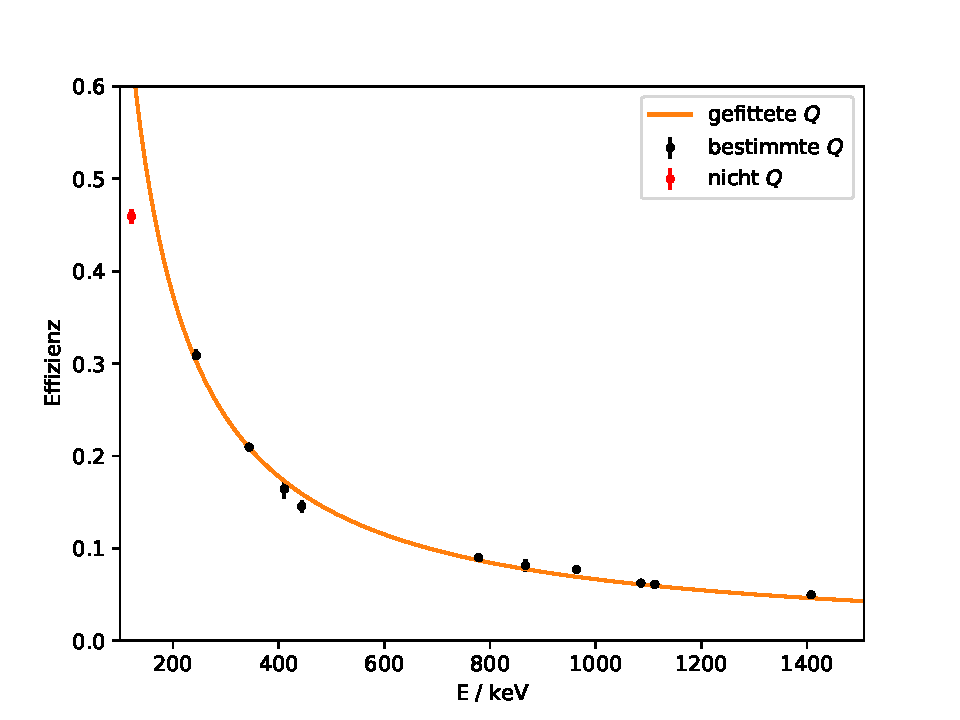
\includegraphics[width = 0.85\textwidth]{Python/Plots/Effizienz.pdf}
  \caption{Berechnete Effizienzen $Q$ sowie die angepasste Potenzfunktion $Q(E)$. }
  \label{fig:Effizienz}
\end{figure}

\subsection{Bestimmung verschiedener Detektoreigenschaften mithilfe einer $^{137}{Cs}$-Quelle }

Durch Aufnahme eines Spektrums der $^{137}{Cs}$-Quelle kann eine Aussage über
die tatsächliche Energieauflösung des Detektors getroffen werden. Zudem kann
durch den Vergleich der Flächen unter dem Compton-Kontinuum sowie des Vollenergiepeaks
eine Aussage über die Wechselwirkungswahrscheinlichkeit getroffen und mit den
theoretischen Werten verglichen werden. Die Messung wurde in einem Zeitraum von
$t\ut{ges} = \SI{3066}{\second}$ durchgeführt.

\subsubsection{Bestimmung der Energieauflösung}
\label{subsubsec:EA}

\begin{figure}
  \centering
  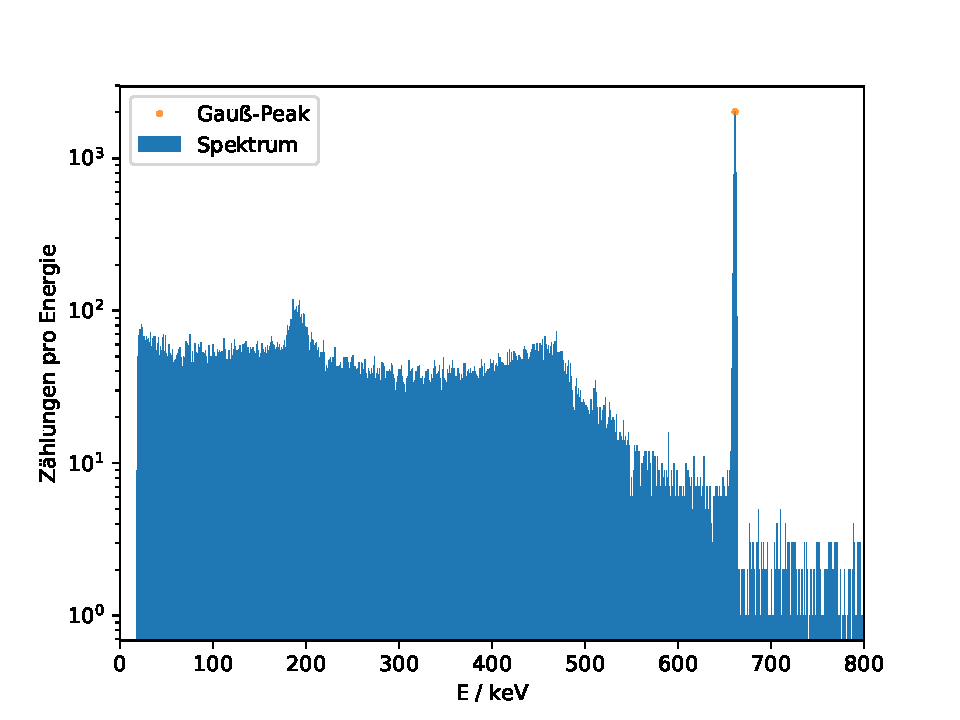
\includegraphics[width=0.85\textwidth]{Python/Plots/Caesium.pdf}
  \caption{Aufgenommenes Spektrum für $^{137}{Cs}$. Der Vollenergiepeak ist farblich markiert.}
  \label{fig:Ca}
\end{figure}
Das aufgenommene Spektrum für $^{137}{Cs}$ ist in Abbildung~\ref{fig:Ca} dargestellt.
Der Vollenergiepeak wurde analog zu Kapitel~\ref{subsubsec:Eu} mithilfe des
\textsc{find\_{peaks}}-Paketes bestimmt und gemäß Formel~\eqref{eqn:Gausfit}
angepasst. Dabei ergeben sich die folgenden Parameter:
\begin{align}
  A &= \SI{2054(13)}{Zählungen} \\
  \mu &= \SI{661.4(2)}{\kilo\eV}
  \label{Ca:mu}\\
  \sigma &= \SI{2.15(2)}{\kilo\eV}
  \label{Ca:sigma}\\
  B &= \SI{6{3}}{Zählungen}.
\end{align}
Der Vollenergiepeak und die angepasste Gauß-Funktion sind in Abbildung~\ref{fig:CaGauß}
dargestellt.
\begin{figure}
  \centering
  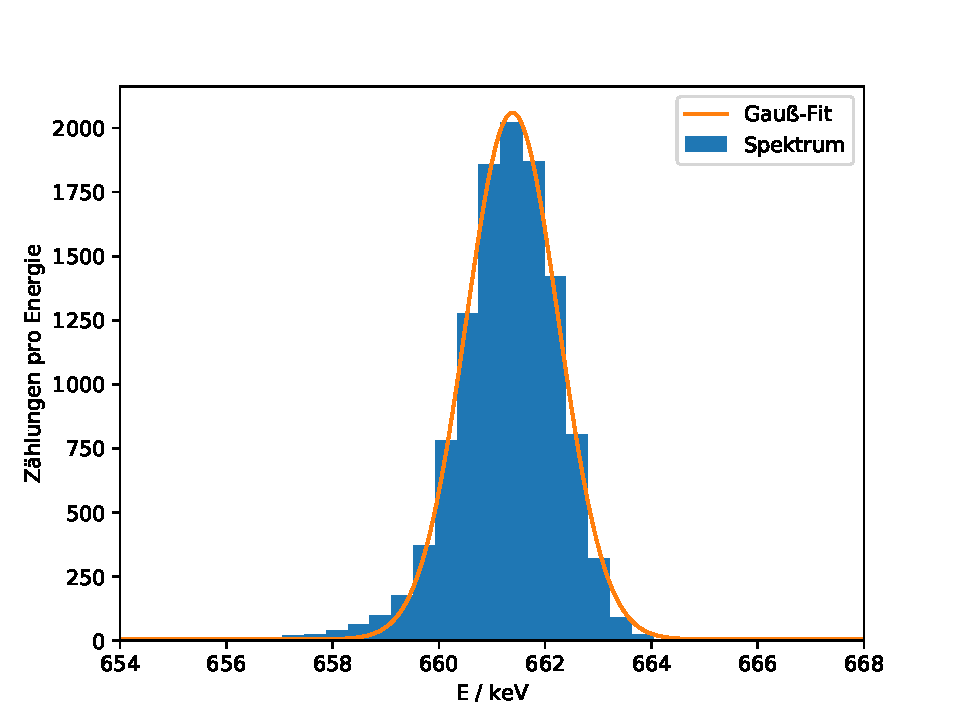
\includegraphics[width=0.85\textwidth]{Python/Plots/Caesium_Gaus.pdf}
  \caption{Angepasste Gaußfunktion für den Vollenergiepeak von $^{137}{Cs}$. }
  \label{fig:CaGauß}
\end{figure}
Um die Verwendung einer Gauß-Funktion als Fitfunktion zu rechtfertigen, wird die
Halbwertsbreite sowie die Zehntelbreite bestimmt. Dafür werden die beiden Energien
gesucht, die die geringste Abweichungen zur Hälfte bzw. dem Zehntel der bestimmten
Amplitude haben. Für die Halbwertsbreite und Zehntelbreite sowie deren Verhältniss
ergibt sich somit:
\begin{align}
  x\ua{1/2} &= \SI{2.4(2)}{\kilo\eV} \\
  x\ua{1/10} &= \SI{4.4(2)}{\kilo\eV} \\
  \frac{x\ua{1/10}}{x\ua{1/2}} &= \SI{1.83(18)}{}.
\end{align}
Beide Breiten können zudem unter Verwendung der bei der Anpassung der Gaußfunktion
bestimmten Standardabweichung~\ref{Ca:sigma} bestimmt werden. Gemäß der Formeln
$x\ua{1/2}~=~\sqrt{8\log{2}}\sigma$ und $x\ua{1/10} = 1.823x\ua{1/2}$
ergeben sich für beide Breiten die Werte
\begin{align}
  x\ua{1/2} &= \SI{2.04(21)}{\kilo\eV} \\
  x\ua{1/10} &= \SI{3.72(21)}{\kilo\eV}.
\end{align}
Mithilfe von Formel~\eqref{eqn:halbwertsbreite} kann auch das theoretische Auflösungvermögen des
Germanium Detektors berechnet werden. Dafür werden die in Kapitel~\ref{subsubsec:Eu}
bestimmte Energie des Vollenergiepeaks und die Anregungsenergie eines
Elektrons in Germanium $E\ua{EL} = \SI{2.9}{\eV}$ benötigt. Für das theoretische
Auflösungsvermögen ergibt sich somit
\begin{equation}
  \increment E\ua{1/2} = \SI{1.0292(1)}{\kilo\eV}.
\end{equation}

\subsubsection{Bestimmung der Wechselwirkungswahrscheinlichkeiten}
\label{subsubsec:P}

Für $^{137}{Cs}$ sollen zudem der Rückstreupeak und die Compton-Kante bestimmt werden
sowie der Quotient der Flächen unter dem Compton-Kontinuum und dem Vollenergiepeak.
Das Compton-Kontinuum und die bestimmten Punkte des Rückstreupeaks und der Compton-Kante
sind in Abbildung~\ref{fig:CaCompton} dargestellt. Die Lage der beiden Punkte kann
aus dem Spektrum mithilfe der \textsc{find\_{peaks}}-Funktion bestimmt werden:
\begin{align}
  E\ut{Rückstreuung} &= \SI{186.2(1)}{\kilo\eV} \\
  E\ut{Kompton-Kante} &= \SI{477.1(1)}{\kilo\eV}.
\end{align}
Zudem können die Energien auch mithilfe von Formeln~\eqref{eqn:comton_E_gamma}
bestimmt werden, so dass sich für die theoretischen Werte
\begin{align}
  E\ut{Rückstreuung} &= \SI{184.3(1)}{\kilo\eV} \\
  E\ut{Kompton-Kante} &= \SI{477.1(1)}{\kilo\eV}
\end{align}
ergibt. Dabei wurde für den Rückstreupeak der Winkel $\Psi = \sfrac{\pi}{2}$ und
für die Compton-Kante der Winkel $\Psi = \pi$ verwendet.
\begin{figure}
  \centering
  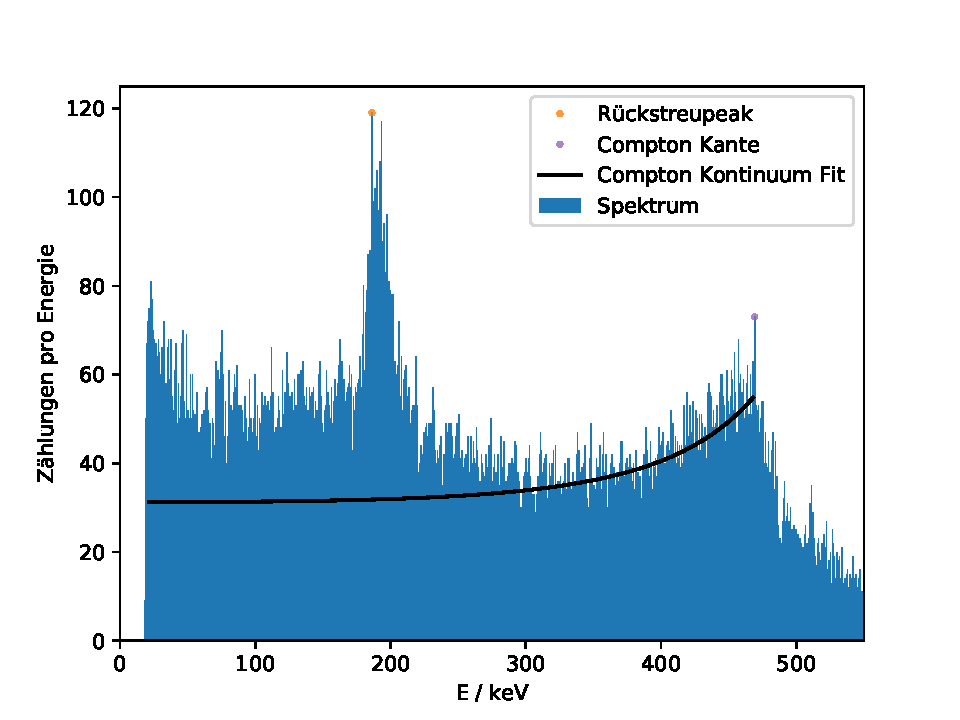
\includegraphics[width=0.85\textwidth]{Python/Plots/Caesium_Compton.pdf}
  \caption{Comptonkontinuum sowie die bestimmte Fitfunktion für $^{137}{Cs}$.
  Der Rückstreupeak sowie die Comptonkante sind farblich markiert.}
  \label{fig:CaCompton}
\end{figure}

Um die Wechselwirkungswahrscheinlichkeit der Comptonstreuung und des Photoeffektes
zu vergleichen, wird im folgenden der Inhalt des Compton-Kontinuums und des Vollenergiepeaks
bestimmt. Bei dem Vollenergiepeak kann dieser analog zu Kapitel~\ref{subsubsec:Eu} mithilfe
der Standardabweichung der Gauß-Fitfunktion \label{Ca:sigma} bestimmt werden:
\begin{equation}
  F\ua{Vollenergie} = \SI{11077(111)}{\text{Zählungen}}.
\end{equation}
Zur Bestimmung des Inhaltes des Compton-Kontinuums werden zwei verschiedene Methoden
verwendet. Die einfachere Methode ist das einfach Aufsummieren aller Zählungen
innerhalb des Compton-Kontinuums. Jedoch wird der Inhalt durch den Rückstreupeak
verfälscht. Deshalb wird in der zweiten Methode eine Anpassung mit einer Funktion
durchgeführt, die dem energieabhängigen Anteil des Wirkungsquerschnittes für die
Comptonstreuung entspricht:
\begin{equation}
  N(x) = N\ua{0} \frac{1}{\varepsilon^2} \cdot \left\{2 + \left(\frac{x}{h\nu-x}\right)^2\cdot\left[\frac{1}{\varepsilon^2}+\frac{h\nu-x}{h\nu}-\frac{2}{\varepsilon}\left(\frac{h\nu-x}{h\nu}\right)\right] \right\}
\end{equation}
Bei $h\nu$ handelt es sich um die Energie des Vollenergiepeaks~\ref{Ca:mu}.
Der konstante Vorfaktor $N\ua{0}$ und das $\varepsilon$ werden
dabei als Fit-Parameter verwendet. Für den Fit wird der Bereich ab einer Energie
von $\SI{400}{\kilo\eV}$ bis zur Comptonkante verwendet.
Der Fit ist in Abbildung~\ref{fig:CaCompton}
dargestellt. Für die beiden Fit-Parameter ergibt sich
\begin{align}
  N\ua{0} &= \SI{58(17)}{\text{Zählungen}} \\
  \varepsilon &= \SI{1.9(3)}{}
\end{align}
Durch Integration über die Energien bis zur Compton-Kante ergibt sich der
Inhalt des Compton-Kontinuums:
\begin{align}
  F\ut{Compton,Summierung} &= \SI{51140(226)}{\text{Zählungen}} \\
  F\ut{Compton,Integration} &= \SI{15719}{Zählungen}
\end{align}
Durch Bestimmung des Quotienten kann später eine Aussage über die relative Wechselwirkungswahrscheinlichkeit
der Comptonstreuung und des Photoeffektes getroffen werden:
\begin{align}
  \frac{F\ut{Compton,Summierung}}{F\ua{Vollenergie}} &= \SI{4.62(5)}{} \\
  \frac{F\ut{Compton,Integration}}{F\ua{Vollenergie}} &= \SI{1.42(1)}{}
\end{align}
Die Quotienten zeigen, dass die Größenordnungen des Inhalts des Compton-Kontinuums
und des Vollenergiepeaks bei beiden Methoden gleich sind.

Die Wechselwirkungswahrscheinlichkeit lässt sich zudem mit der Formel
\begin{equation}
  P = (1 - e^{-\mu d})\cdot 100
\end{equation}
berechnen, wobei es sich bei $\mu$ um den Extinktionskoeffizienten und bei $d$ um
die Dicke der Probe handelt. Dafür müssen die Extinktionskoeffiienzenten aus Quelle \cite{anleitung}
entnommen werden. Aufgrund der logarithmischen Darstellung werden unterschiedliche
Ablesefehler angenommen:
\begin{align}
  \mu\ut{Photo} &= \SI{8(1)e-3}{\per\cm} \\
  \mu\ut{Compton} &= \SI{0.37(1)}{\per\cm}
\end{align}
Für die Wechselwirkungswahrscheinlichkeiten sowie den Quotienten ergibt sich somit
\begin{align}
  P\ua{Photo} &= \SI{3.1(4)}{\percent} \\
  P\ua{Compton} &= \SI{76.4(9)}{\percent} \\
  \frac{P\ua{Compton}}{P\ua{Photo}} &= \SI{25(3)}{}
\end{align}
Der Quotient der Wechselwirkungswahrscheinlichkeiten ist deutlich größer als
der Quotient der beiden Flächen.

\subsection{Untersuchung der ersten unbekannten Quelle}
\label{subsec:u1}

\begin{figure}
  \centering
  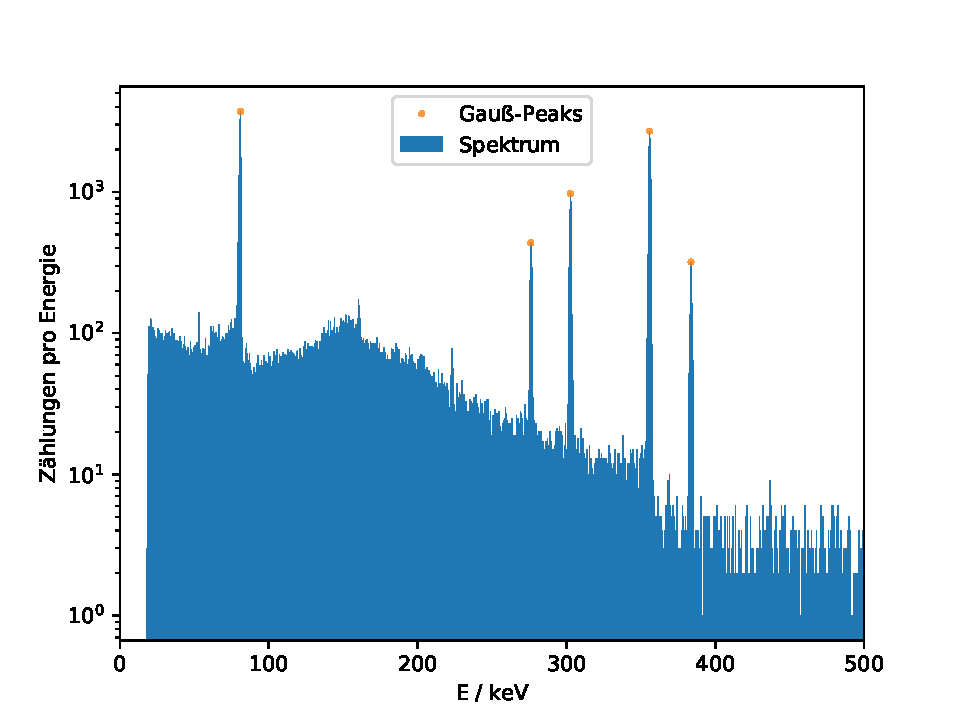
\includegraphics[width = 0.85\textwidth]{Python/Plots/unbekannt1.pdf}
  \caption{Aufgenommenes Spektrum für die 1. unbekannte Quelle. Die bestimmten
  Vollenergiepeaks sind farblich markiert.}
  \label{fig:u1}
\end{figure}
Das aufgenommene Spektrum für die erste unbekannte Quelle ist in Abbildung~\ref{fig:u1}
dargestellt. Die Messzeit betrug $t\ut{ges} = \SI{3066}{\second}$.
Ein Vergleich der Energien der analog zu dem vorherigen Kapiteln bestimmten Peaks
mit den in Quelle \cite{anleitung} gegebenen $E_{\gamma,\su{lit}}$ von $^{133}{Ba}$
und $^{125}{Sb}$ zeigt, dass es sich bei der untersuchten Quelle um $^{133}{Ba}$
handelt. Die aus der Anpassung an die Gaußfunktion~\ref{eqn:Gausfit} erhaltenen
Parameter sind in Tabelle~\ref{tab:u1} aufgelistet. Die bestimmten Mittelwerte
bzw. Energien der einzelnen Peaks sind in Abbildung~\ref{fig:u2} markiert.
\begin{table}
  \centering
  \caption{Die bestimmten Parameter aus dem Fit mit der Gaußfunktion sowie
  die zugeordneten Energien aus der Literatur für $^{133}{Ba}$.}
  \label{tab:u1}
  \begin{tabular}{S[table-format=3] S[table-format=4]@{${}\pm{}$} S[table-format=2]
    S[table-format=3.1]@{${}\pm{}$} S[table-format=1.]
    S[table-format=1.2]@{${}\pm{}$} S[table-format=1.2]
    S[table-format=2.0]@{${}\pm{}$} S[table-format=1.] S[table-format=3.1]}
    \toprule
    {Kanal} & \multicolumn{2}{c}{$A$ / Zählung} & \multicolumn{2}{c}{$\mu$ / Kanal}
    & \multicolumn{2}{c}{$\sigma$ / Kanal} & \multicolumn{2}{c}{$B$ / Zählung}
    & {$E_{\gamma,\su{lit}}$ / $\si{\kilo\eV}$} \\
    \midrule
    208 & 3785 & 56 &  80.9 & 0.1 & 1.08 & 0.01 & 93 & 9 &  81.0 \\
    693 &  447 &  5 & 276.3 & 0.1 & 1.36 & 0.02 & 18 & 1 & 276.4 \\
    758 &  991 &  7 & 302.8 & 0.1 & 1.42 & 0.01 & 14 & 1 & 302.9 \\
    890 & 2742 & 12 & 355.9 & 0.1 & 1.51 & 0.01 &  8 & 2 & 356.0 \\
    959 &  337 &  4 & 383.8 & 0.1 & 1.58 & 0.02 &  3 & 1 & 383.9 \\
    \bottomrule
  \end{tabular}
\end{table}


Um die Aktvität der $^{133}{Ba}$-Quelle zu bestimmen, müssen zuerst die Flächen
unter den einzelnen Peaks bestimmt werden sowie die jeweilige Effizienz. Der Raumwinkel
wurde schon in Abschnitt~\ref{subsubsec:Eff} bestimmt. Die
Bestimmung beider Größen wird mithilfe der in Kapitel~\ref{subsubsec:Eff}
angegebenen Formel für eine Gaußfunktion~\ref{eqn:area} sowie der bestimmten
Formel für die Effizienz~\ref{eqn:eff} durchgeführt. Die Übergangswahrscheinlichkeiten
können Quelle \cite{anleitung} entnommen werden. Alle verwendeten Messgrößen sowie
die durch Umstellen von Formel~\eqref{eqn:effizienz} bestimmten Aktivitäten sind in Tabelle~\ref{tab:u1Aktivität} eingetragen.
Unter Berücksichtigung aller Messdaten ergibt sich für die gemittelte
Aktivität $A\ua{^{133}{Ba}} = \SI{1073(306)}{\becquerel}$. Aufgrund der großen Abweichung
der Aktivität des Peaks bei einer Energie von $\SI{80.9(1)}{\kilo\eV}$ wird
auch der Mittelwert ohne diesen Messwert berechnet. Dabei ergibt sich eine gemittelte
Akitvität von $A\ua{^{133}{Ba}} = \SI{1228(351)}{\becquerel}$.
\begin{table}
  \centering
  \caption{Die bestimmmten Parameter für Formel \eqref{eqn:effizienz} und die daraus resultierenden Aktivitäten
          für $^{133}{Ba}$.}
  \label{tab:u1Aktivität}
  \begin{tabular}{S[table-format=3.1]@{${}\pm{}$}S[table-format=1.1]
                  S[table-format=5.]@{${}\pm{}$}S[table-format=3.]
                  S[table-format=1.3]
                  S[table-format=1.2]@{${}\pm{}$}S[table-format=1.2]
                  S[table-format=4.]@{${}\pm{}$}S[table-format=3.]}
    \toprule
    \multicolumn{2}{c}{$E_{\gamma, \text{exp}} $ / $\si{\kilo\eV}$} &
    \multicolumn{2}{c}{$F\ua{Peak}$ / Zählungen} &
    {W } & \multicolumn{2}{c}{$Q$} & \multicolumn{2}{c}{$A$ / $\si{\becquerel}$}\\
    \midrule
     80.9 & 0.1 & 10316 & 237 & 0.341 & 0.99 & 0.25 &  464 & 119 \\
    276.3 & 0.1 &  1520 &  24 & 0.072 & 0.26 & 0.08 & 1210 & 343 \\
    302.8 & 0.1 &  3531 &  38 & 0.183 & 0.24 & 0.07 & 1219 & 348 \\
    355.9 & 0.1 & 10376 &  66 & 0.621 & 0.20 & 0.06 & 1255 & 364 \\
    383.8 & 0.1 &  1331 &  22 & 0.089 & 0.19 & 0.05 & 1218 & 355 \\
    \bottomrule
  \end{tabular}
\end{table}


\subsection{Untersuchung der zweiten unbekannten Quelle}

\begin{figure}
  \centering
  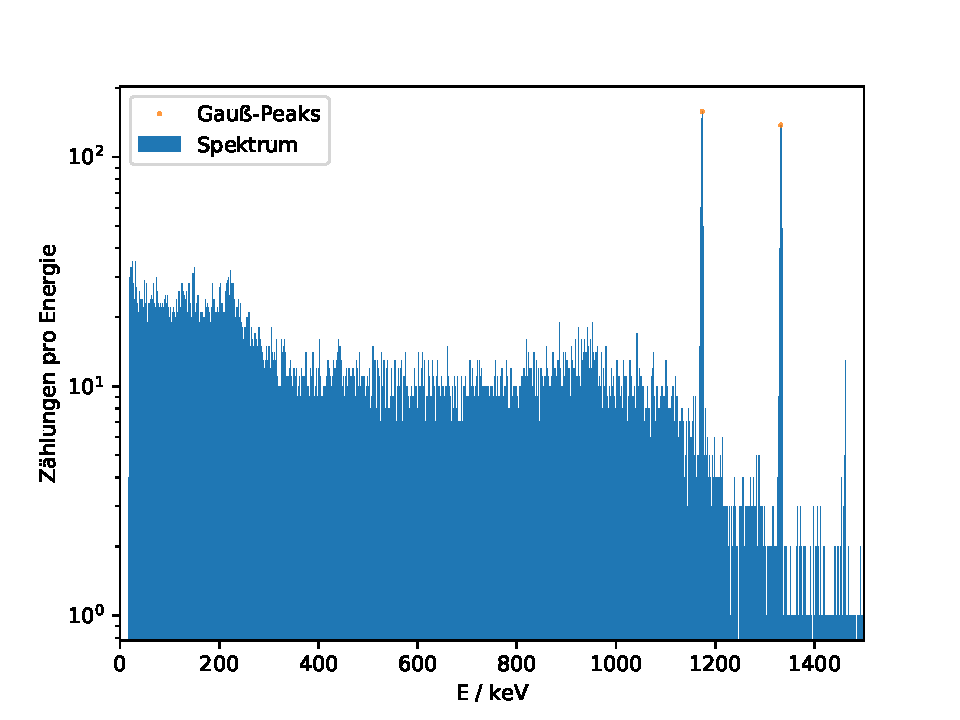
\includegraphics[width=0.85\textwidth]{Python/Plots/unbekannt2.pdf}
  \caption{Aufgenommenes Spektrum für die 2. unbekannte Quelle. Die bestimmten
  Vollenergiepeaks sind farblich markiert.}
  \label{fig:u2}
\end{figure}
Für die zweite unbekannte Quelle wird analog zu der in Kapitel~\ref{subsec:u1}
behandelten unbekannten Quelle vorgegangen. Das aufgenommene Spektrum ist in
Abbildung~\ref{fig:u2} dargestellt und wurde in einem Zeitraum von
 $t\ut{ges} = \SI{4046}{\second}$ aufgenommen. Die bestimmten Energien der beiden Vollenergiepeaks
sind zudem grafisch markiert. Ein Vergleich mit verschiedenen Atomen zeigt, dass
es sich bei dieser Quelle um $^{60}{Co}$ handelt \cite{cobalt}. Die aus dem
der Anpassung bestimmten Parameter sind in Tabelle~\ref{tab:u2} eingetragen.
\begin{table}
  \centering
  \caption{Die bestimmten Parameter aus dem Fit mit der Gaußfunktion sowie
  die zugeordneten Energien aus der Literatur für $^{60}{Co}$.}
  \label{tab:u2}
  \begin{tabular}{S[table-format=4] S[table-format=3]@{${}\pm{}$} S[table-format=1]
    S[table-format=4.1]@{${}\pm{}$} S[table-format=1.1]
    S[table-format=1.2]@{${}\pm{}$} S[table-format=1.2]
    S[table-format=1.1]@{${}\pm{}$} S[table-format=1.1] S[table-format=4.2]}
    \toprule
    {Kanal} & \multicolumn{2}{c}{$A$ / Zählung} & \multicolumn{2}{c}{$\mu$ / Kanal}
    & \multicolumn{2}{c}{$\sigma$ / Kanal} & \multicolumn{2}{c}{$B$ / Zählung}
    & {$E_{\gamma,\su{lit}}$ / $\si{\kilo\eV}$}\\
    \midrule
    2918 & 149 & 3 & 1173.1 & 0.2 & 3.40 & 0.09 & 3.0 & 0.9 & 1173.24 \\
    3313 & 137 & 2 & 1332.3 & 0.2 & 3.46 & 0.06 & 1.2 & 0.6 & 1332.50 \\
    \bottomrule
  \end{tabular}
\end{table}


Zur Bestimmung der Aktivität werden auch bei dieser Quelle die verschiedenen
Peakflächen sowie die Effizienzen analog zu Kaptel~\ref{subsec:u1} bestimmt.
Die Übergangswahrscheinlichkeiten werden Quelle \cite{cobalt} entnommen.
Die verschiedenen Größen sowie die bestimmten Aktivitäten sind in Tabelle
\ref{tab:u2Aktivität} eingetragen. Für die gemittelte Aktivität ergibt sich ein
Wert von $A\ua{^{60}{Co}} = \SI{377(121)}{\becquerel}$.
\begin{table}
  \centering
  \caption{Die bestimmmten Parameter für Formel \eqref{eqn:effizienz} und die daraus resultierenden Aktivitäten
          für $^{60}{Co}$.}
  \label{tab:u2Aktivität}
  \begin{tabular}{S[table-format=4.1]@{${}\pm{}$} S[table-format=1.1]
                  S[table-format=4.]@{${}\pm{}$} S[table-format=2.]
                  S[table-format=2.2]  S[table-format=1.2]@{${}\pm{}$}
                  S[table-format=1.2] S[table-format=3.]@{${}\pm{}$}
                  S[table-format=3.]} \\
    \toprule
    \multicolumn{2}{c}{$E_{\gamma, \text{exp}} $ / $\si{\kilo\eV}$} &
    \multicolumn{2}{c}{$F\ua{Peak}$ / Zählungen} &
    {W } & \multicolumn{2}{c}{$Q$} & \multicolumn{2}{c}{$A$ / $\si{\becquerel}$}\\
    1173.1 & 0.2 & 1270 & 44 & 99.97 & 0.06 & 0.02 & 364 & 117 \\
    1332.3 & 0.2 & 1190 & 25 & 99.99 & 0.05 & 0.02 & 390 & 126 \\
    \bottomrule
  \end{tabular}
\end{table}


\newpage
\section{Diskussion}

In Kapitel~\ref{subsubsec:Eu} wurde mittels der gefundenen Peaks und einigen Literaturwerten
die Kalibrierung des Detektors bzw. die Bestimmung der Transformation für die Kanäle
in die jeweiligen Energien durchgeführt. Die Fehler der bestimmten Parameter
sind ziemlich gering. Die Genauigkeit lässt sich zudem durch die
verschiedenen Proben bestätigen, da die Abweichungen der experimentell bestimmten
Energien von den Literaturwerten durchgehend unter $\SI{1}{\percent}$ liegen.

Bei der Bestimmung der Potenzfunktion für die Effizienz in Abhängigkeit der Energie
zeigt sich besonders bei der Amplitude ein großer relativer Fehler von knapp
$\SI{21}{\percent}$. Besonders bei der Bestimmung der Aktivität von $^{60}{Co}$
zeigt sich für den Peak bei
einer Energie von $\SI{80.9}{\kilo\eV}$ eine starke Abweichung gegnüber den anderen
Energien. Diese Abweichung ist schon bei der Effizienz erkennbar. In Kapitel
\ref{subsubsec:Eff} werden nur Werte für Energien über $\SI{150}{\kilo\eV}$ zur
Bestimmung der Effizienz verwendet. In Abbildung~\ref{fig:Effizienz} ist erkenntlich,
dass die angepasste Potenzfunktion schon bei einer Energie von $\SI{121.76}{\kilo\eV}$
starke Abweichungen gegenüber des berechneten Wertes zeigt. Dies rechtfertigt eine
Berechnung der gemittelten Aktivität ohne Berücksichtigung des stark abweichenden
Wertes.

In Kapitel~\ref{subsubsec:EA} wurde die Halbwertsbreite bzw. das Auflösungsvermögen
des Detektors anhand der aufgenommenen Spektren bestimmt. Das Verhältniss von
Halbwertsbreite zur Zehntelbreite zeigt, dass die Annahme einer Gauß-Verteilung
gerechtfertigt ist. Im Vergleich zur theoretischen Energieauflösung ist der
experimentell bestimmte Wert jedoch ungefährt doppelt so groß. Dies liegt vermutlich
an verschiedenen Verbreiterungsmechanismen aufgrund der elektrischen Schaltung etc. .

Bei Betrachtung der Wechselwirkungswahrscheinlichkeiten von Comptonstreuung und
Photoeffekt in Kapitel~\ref{subsubsec:P} zeigen sich deutliche Unterschiede
bei den verwendeten Methoden. Bei Berechnung des Quotienten beider
Wechselwirkungswahrscheinlichkeiten mittels der Extinktionskoeffizienten
ist die Wahrscheinlichkeit für die Comptonstreuung um den Faktor 25 größer als
für den Photoeffekt. Bei Vergleich der Flächen des Compton-Kontinuums und des
Vollenergiepeaks ergibt sich jedoch lediglich ein Faktor von $\num{1.42}$
bzw. $\num{4.62}$. Dies liegt daran, dass bei Verwendung der Extinktionskoeffizienten
lediglich der 1-fache Photoeffekt berüchsichtigt wird. Jedoch können auch mehrfach
comptongestreute Photonen bei genügend Energie über den Photoeffekt wechselwirken.
Zudem wird der Extinktionskoeffizient für den Photoeffekt mit abnehmender Energie
größer (siehe Abbildung~\ref{fig:crosssection}). Dies sorgt für eine deutliche
Vergößerung der Fläche unter dem Vollenergiepeak. Die starken Unterschiede der
Flächenverhältnisse bei den verschiedenen Methoden lassen sich dadurch erklären,
dass bei dem verwendeten Fit neben den Zählungen innerhalb des Rückstreupeaks
im niedrigen Energiebereich auch ein großer Teil der Compton-Kontinuums
abgeschnitten wird.

Im Allgemeinen zeigt die Bestimmung der beiden unbekannten Quellen mit sehr hoher
Genauigkeit, dass der verwendete Germaniumdetektor sehr präzise ist.
